\chapter{让有质量的机器人跟上轨迹}
\begin{notebox}
\textbf{目标}\quad 从参考 p/v/a 计算真实力与力矩，区分反馈、前馈、模型失配和饱和。\\
\textbf{先修}\quad 第 04、14 章；本章参考已给定，先隔离跟踪问题。
\end{notebox}
\section{位置不是受力模型的控制量}
\begin{lstlisting}[language=bash]
ros2 run motion2d pd_tracking_demo tmp/ch17_pd
/usr/bin/python3 scripts/plot_ch17_pd.py
\end{lstlisting}
理想执行直接取参考位置。有质量的机器人满足 $m\dot v=F-c_vv$，
即使立刻改变力，速度和位置也不会瞬间跳到目标。
控制器从同一 odom 坐标系读取当前位置/速度及参考 p/v/a，先求期望加速度，再换算成力：
\begin{equation}
 e_p=p_r-p,\qquad e_v=v_r-v,\qquad
 F=\hat m(a_r+K_pe_p+K_de_v)+\hat c_vv.
\end{equation}
帽子表示控制器使用的参数估计；它不应悄悄读取模拟器真值参数。
$a_r$ 是前馈：提前提供沿曲线运动所需的加速度。
位置项把偏离拉回，速度项减小来回振荡；$K_p$ 单位为 s$^{-2}$，$K_d$ 为 s$^{-1}$。

\section{独立 yaw 与执行器限幅}
yaw 误差使用最短包角差，角速度误差按 rad/s 计算；再用转动惯量和角阻力换算力矩。
本章圆盘可全向受力，yaw 不决定平移方向；差速轮式车是另一种动力学模型。
\lstinputlisting[language=C++,linerange={pd_force_begin-pd_force_end},
 includerangemarker=false]{../ros2_ws/src/motion2d/src/control/pd_tracker.cpp}
trackPd 同时返回 requested 和 applied，方便看出要求了多少、实际执行了多少。
每个力轴分别限制在 $[-F_{\max},F_{\max}]$，力矩同理；没有把状态速度硬裁掉。
若力饱和，机器人可能跟不上轨迹，轨迹应减速或重新分配时间。

\clearpage
\section{固定参考后，比较原因而非只看最终位置}
实验使用空 8 m 方形边界、半径 0.2 m 圆盘；净空由边界到圆盘外缘的距离计算，
仅用于评估，不输入控制器。实际质量 1 kg、线阻力 0.15 kg/s、转动惯量 0.02 kg\,m$^2$、角阻力 0.01；
两轴 $K_p=4,K_d=3$，yaw 同值。每次运行 24 s，动力学 200 Hz、控制 50 Hz，命令在四个动力学步内保持。
这是无通信延迟的核心实验，ROS 链路的表现单独验收。

\begin{figure}[!ht]
\centering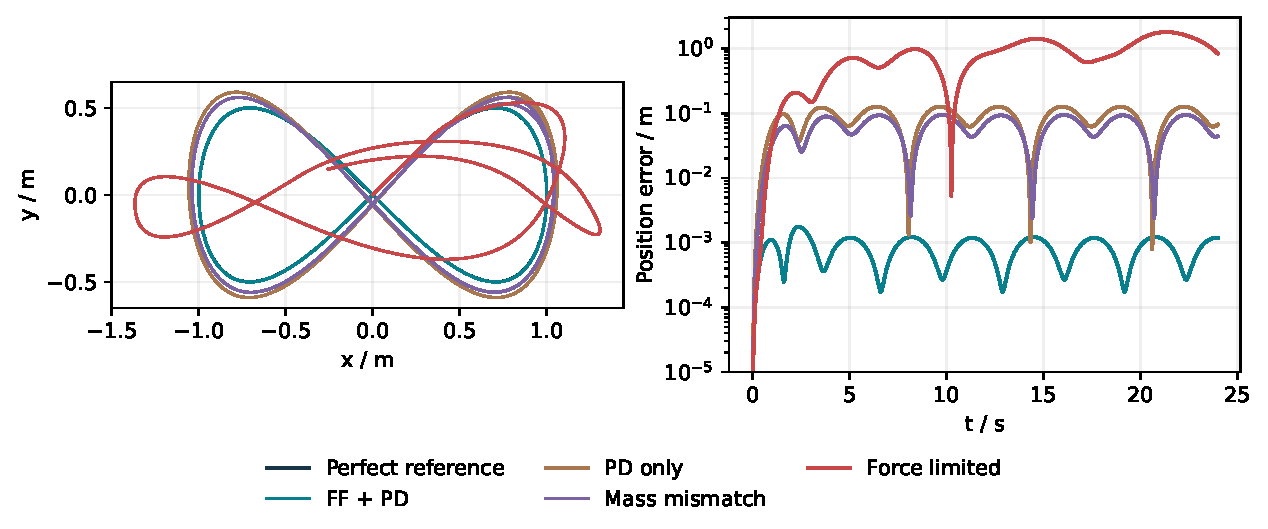
\includegraphics[width=\linewidth]{figures/ch17_pd.pdf}
\caption{八字参考上的几何路线与位置误差。误差纵轴为对数，范围下方的早期值不显示；
理想参考误差为零，不画在对数轴上。每轴 0.2 N 限力导致明显跟踪失败，即使场景仍有足够净空。}
\end{figure}

\begin{center}\small
\begin{tabular}{lrr}\toprule
控制条件 & 圆形 RMS/m & 八字 RMS/m\\\midrule
前馈 + PD，模型匹配 & 0.000393 & 0.000898\\
关闭加速度前馈 & 0.06112 & 0.09151\\
估计质量 0.6 kg & 0.04262 & 0.06691\\
每轴力限 0.2 N & 0.97127 & 0.95082\\\bottomrule
\end{tabular}
\end{center}
关闭前馈仍保留阻力补偿；质量失配组同时将估计转动惯量改为 0.012 kg\,m$^2$。
其他动态组的每轴力限为 2 N、力矩限为 0.2 N\,m。
完整 CSV 还记录最大位置误差、yaw RMS、输入峰值、最小净空和饱和控制次数。
模型匹配的八字实际每轴力峰值约 0.508 N；限力组最大位置误差约 1.802 m。
理想模式直接采样参考，位置误差为零；其力峰值记 NaN，避免误解成“零牛顿也能完成运动”。

\clearpage
\section{参考要平滑起步，不能凭空跳出速度}
直接令相位 $\theta=\omega t$，圆轨迹起点已带速度；本章将相位时钟平滑启动。
给定渐入时长 $R=2$ s，在 $s=t/R\in[0,1]$ 时使用
\begin{equation}
 \tau=R(s^3-\tfrac12s^4),\quad \dot\tau=3s^2-2s^3,\quad
 \ddot\tau=6s(1-s)/R;\qquad \theta=\omega\tau.
\end{equation}
$t\geq R$ 后 $\tau=t-R/2$、$\dot\tau=1$、$\ddot\tau=0$，因此起点静止，连接处 p/v/a 连续。
局部坐标下两种路线分别为
\begin{equation}
 p_{\rm circle}(\theta)=r\begin{bmatrix}\sin\theta\\1-\cos\theta\end{bmatrix},\qquad
 p_{\rm eight}(\theta)=r\begin{bmatrix}\sin\theta\\\tfrac12\sin2\theta\end{bmatrix}.
\end{equation}
用链式法则计算 $v=p_\theta\dot\theta$、$a=p_{\theta\theta}\dot\theta^2+p_\theta\ddot\theta$，
再按参考初始 yaw 旋转到 odom。独立朝向为 $\psi=\psi_0+0.4\sin(\theta/2)$，角速度/角加速度也解析求导。
默认 $r=1$ m、$\omega=0.5$ rad/s；参考尺度与机器人碰撞半径是两件事。

\section{验证、制动与练习}
模型精确、无饱和、理想连续反馈时，可将控制律代入得到
\begin{equation}
 \ddot e_p+K_d\dot e_p+K_pe_p=0.
\end{equation}
此式解释增益作用，却不能直接证明有采样延迟和输入饱和时仍按同样规律收敛。

测试零误差时前馈对应的实际加速度，检查质量和阻力的单位；验证跨 $\pm\pi$ 的 yaw 误差，
检查限幅及阻尼制动力始终反向做功。圆形/八字的 p/v/a 与角导数用中心差分检查，包含渐入连接点。
这些检查验证控制实现的意义，而不只是图看起来贴合。

dampingBrake 按当前速度给出 $F=-\hat m k_bv$、$\tau=-\hat I_zk_b\omega$ 并限幅。
它产生一个新的制动命令，后续 MPC 失败时不会继续发送旧优化结果。
制动需要时间和距离，不代表能在任何障碍前停下，也不自动满足输入变化率限制。

\begin{enumerate}
\item \textbf{推导：}去掉加速度前馈时，误差方程右侧多出什么？模型质量估计偏小时又如何变化？
\item \textbf{代码 ch17-1：}补全逐轴力限幅，解释它和向量范数缩放为什么不同。
\item \textbf{实验：}同样参考依次改变质量估计、阻力和力上限；报告 RMS、最大误差、力峰值与净空，
不能只说“增益更大所以更稳定”。
\end{enumerate}
